
\begin{figure}[t]
\captionsetup[subfloat]{aboveskip=1pt,belowskip=1pt}
    \centering
    
\includegraphics[width=5.5in]{submissions/Jing2024/figures/experiments/evaluation_scores/legend_abla.pdf}\\
     \vspace{-5mm}
    \subfloat[LLaMA 7B]{
        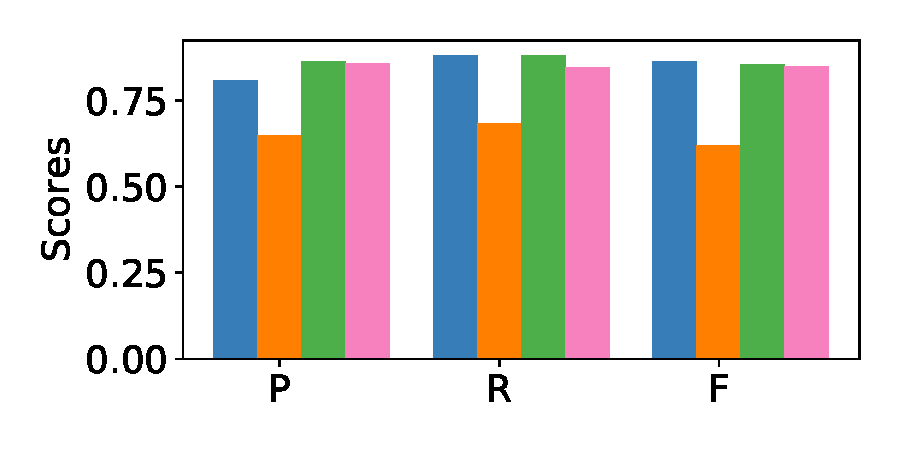
\includegraphics[width=1.78in]{submissions/Jing2024/figures/experiments/evaluation_scores/evaluation_scores_llama_2_7b.pdf}
        \label{fig:evaluation_scores_llama_2_7b}
       }\hspace{-4mm}
    \subfloat[LLaMA 13B]{
        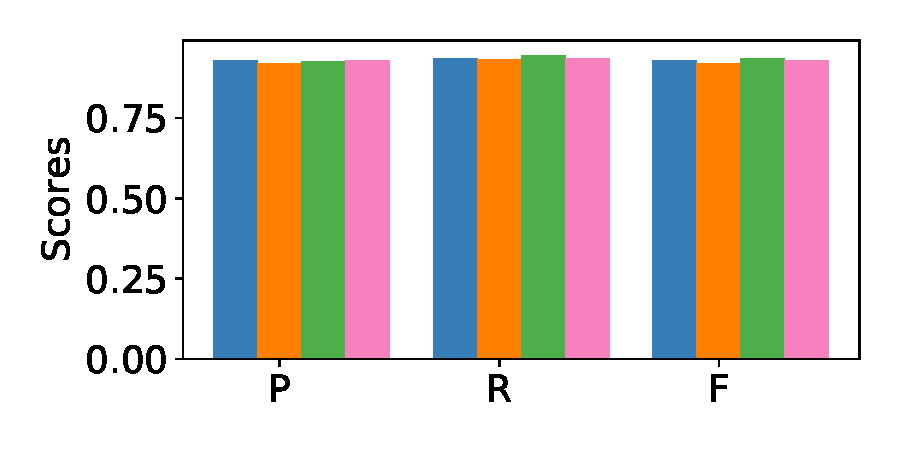
\includegraphics[width=1.78in]{submissions/Jing2024/figures/experiments/evaluation_scores/evaluation_scores_llama_2_13b.pdf}
        \label{fig:evaluation_scores_llama_2_13b}
       }\hspace{-4mm}
    \subfloat[LLaMA 70B]{
        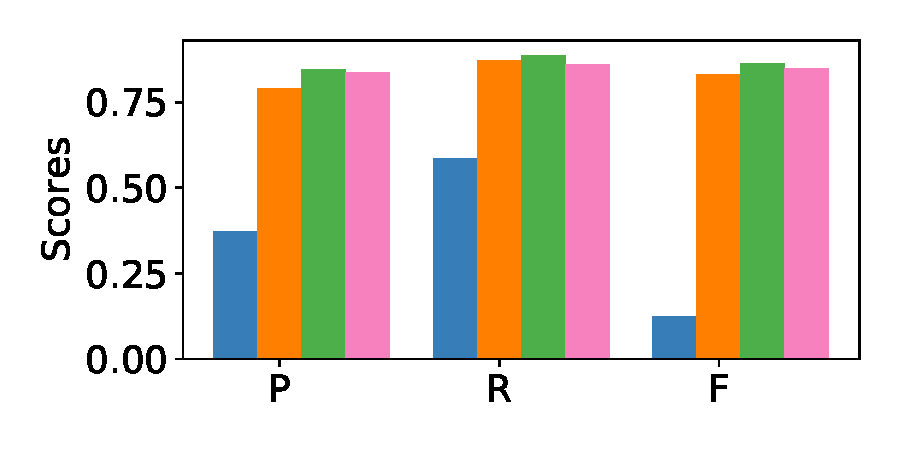
\includegraphics[width=1.78in]{submissions/Jing2024/figures/experiments/evaluation_scores/evaluation_scores_llama_2_70b.pdf}
        \label{fig:evaluation_scores_llama_2_70b}
       }
    \\\vspace{-4mm}
    \subfloat[Gemma 2B]{
        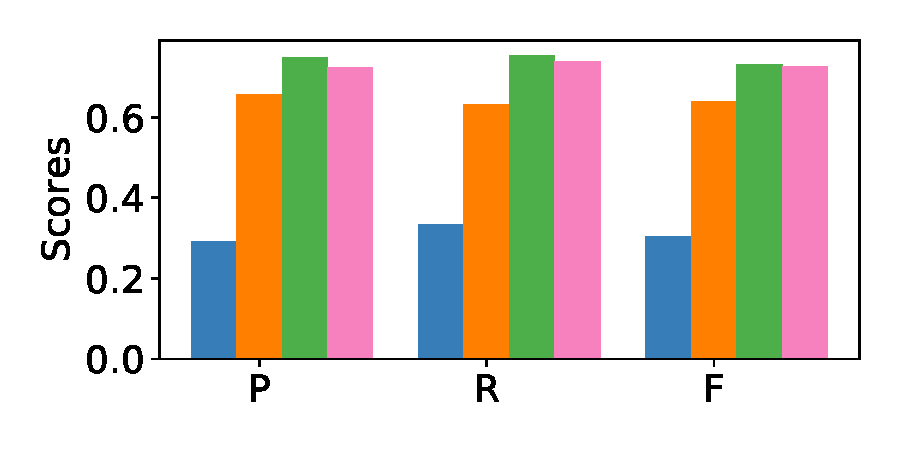
\includegraphics[width=1.78in]{submissions/Jing2024/figures/experiments/evaluation_scores/evaluation_scores_gemma_2b.pdf}
        \label{fig:evaluation_scores_gemma_2b}
       }\hspace{-4mm}
    \subfloat[Gemma 7B]{
        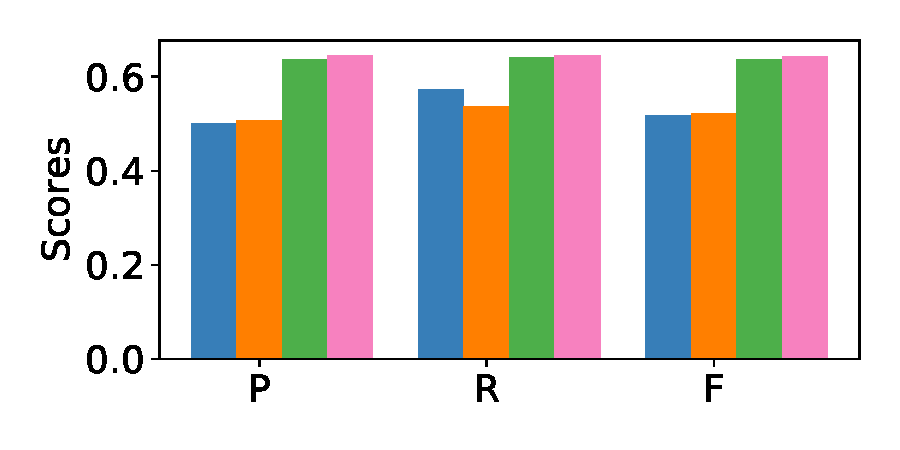
\includegraphics[width=1.78in]{submissions/Jing2024/figures/experiments/evaluation_scores/evaluation_scores_gemma_7b.pdf}
        \label{fig:evaluation_scores_gemma_7b}
       }\hspace{-4mm}
    \subfloat[Average]{
        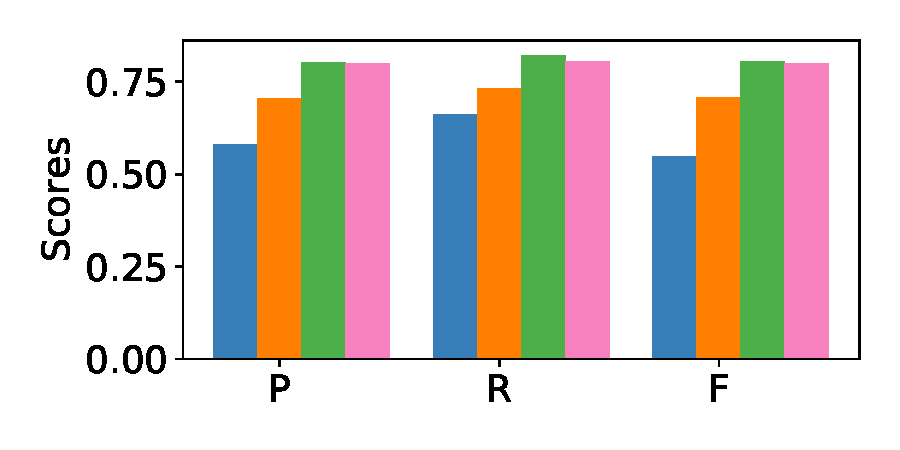
\includegraphics[width=1.78in]{submissions/Jing2024/figures/experiments/evaluation_scores/evaluation_scores_average.pdf}
        \label{fig:evaluation_scores_average}
       }
       \vspace{-3mm}
    \caption{Evaluation scores on the judge model's performance on the labeled validation set. P, R, and F are Precision, Recall, and F1 Score. 
    }
    \vspace{-3mm}
    \label{fig:evaluation_scores}
\end{figure}
